\documentclass{scrartcl}

\usepackage[utf8]{inputenc}


% zus�tzliche mathematische Symbole, AMS=American Mathematical Society 
\usepackage{amssymb}
\usepackage{amsmath}
\usepackage{amsthm}
\usepackage{bbm}
\usepackage{color}
\usepackage{listings}
\usepackage{pdfpages}
\usepackage{csquotes}
\usepackage{float}

% f�rs Einbinden von Graphiken
\usepackage{graphicx}

% f�r Namen etc. in Kopf- oder Fu�zeile
\usepackage{fancyhdr}
\usepackage{tikz}
\usetikzlibrary{arrows, automata}

% erlaubt benutzerdefinierte Kopfzeilen 
\pagestyle{fancy}

% Definition der Kopfzeile
\lhead{
\begin{tabular}{lll}
Maciej Janowski \\
\end{tabular}
}
\chead{}
\rhead{\today{}}
\lfoot{}
\cfoot{Seite \thepage}
\rfoot{} 

\begin{document}

\section*{LAB}
\subsection*{Task}
Our task was to complete the given code implementing the fully connected neural network with the forward propagation and backward propagation algorithms. 

\subsection*{Parameters}
After completing the code I have introduced some experiments. I got best results using learning rate as 0.1 and parameters for each layer shown in the table below. 


\begin{table}[h]
	\centering
\begin{tabular}{|c||c|c|}
	\hline
	\textbf{Layer} & \textbf{Activation function} & \textbf{Number of neurons} \\ \hline \hline
	1st & ReLu & 80 \\ \hline
	2nd & Tanh  & 70  \\ \hline
	3rd & None  & 10  \\ \hline
\end{tabular}
\caption{Parameters for each layer}
\end{table}

\subsection*{Results}
With presented parameters, the graphs of validation and train loss are shown below. 
\begin{figure}[H]
	\centering
	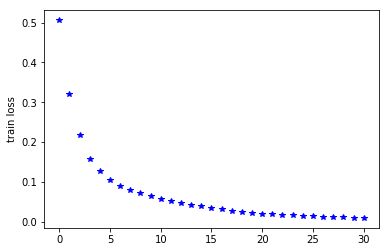
\includegraphics[scale=0.6]{train_loss}
	\caption{Train loss graph}
	\label{fig:trainLost}
\end{figure}

\begin{figure}[H]
	\centering
	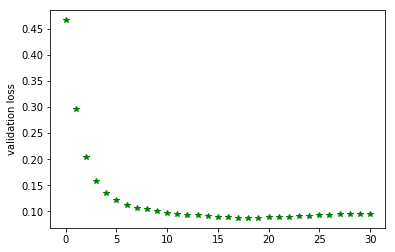
\includegraphics[scale=0.6]{validation_loss}
	\caption{Validation loss graph}
	\label{fig:validationLost}
\end{figure}

After 30 epochs validation error is about 2.2 and duration about 95s.

\subsection*{Comments}
Aka problems that I have faced:
\begin{itemize}
	\item I spent more than 10 hours on that project. I think, mostly because I am not that familiar with Python. Unfortunately, I was not able to code dropout and regularization. 
	\item Really hard was also to find the best performing parameters. In my last project, I used a genetic algorithm to find them, however, I could not find time to apply it.
\end{itemize}
\end{document}


